本アプリのUI設計を以下に示す。
\subsection{依頼側}
\subsubsection{お問い合わせ送信}
\begin{figure}[H]
  \centering
  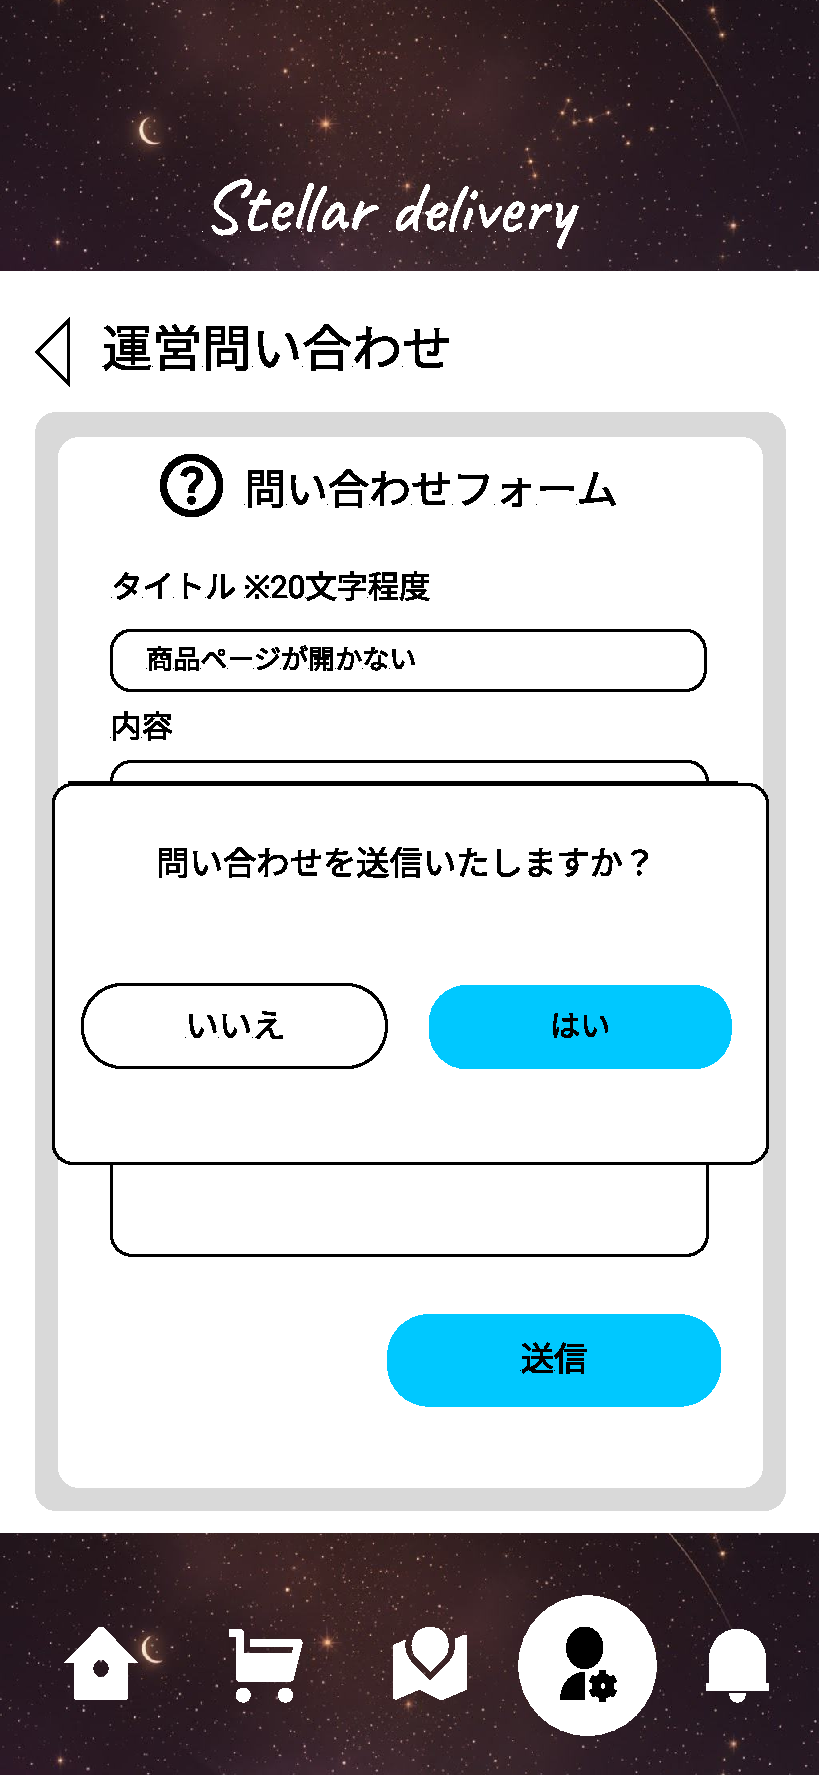
\includegraphics[width=0.75\textwidth]{./pic/customer画面デザイン/お問い合わせ送信.pdf}
  \caption{お問い合わせ送信}
  \label{fig:お問い合わせ送信}
\end{figure}
\subsubsection{マイページ}
\begin{figure}[H]
  \centering
  \includegraphics[width=0.75\textwidth]{./pic/customer画面デザイン/マイページ.pdf}
  \caption{マイページ}
  \label{fig:マイページ}
\end{figure}

\subsection{配達側}
\subsection{配達側}
\subsubsection{ログイン画面}
利用者がStellardeliveryのサイトにアクセスするために、ログイン画面および図\ref{fig:ログイン画面}にてIDとパスワードの入力を行う。この際に、アカウントがない場合は、ログインボタンの上記にある新規会員登録画面へ遷移するリンクを選択することで新規会員登録画面に移行する。また、IDおよびパスワードを入力するテキストボックスの下記にあるリンクを選択することでIDおよびパスワードを忘れた場合の処置が可能となっている。
\begin{figure}[H]
  \centering
  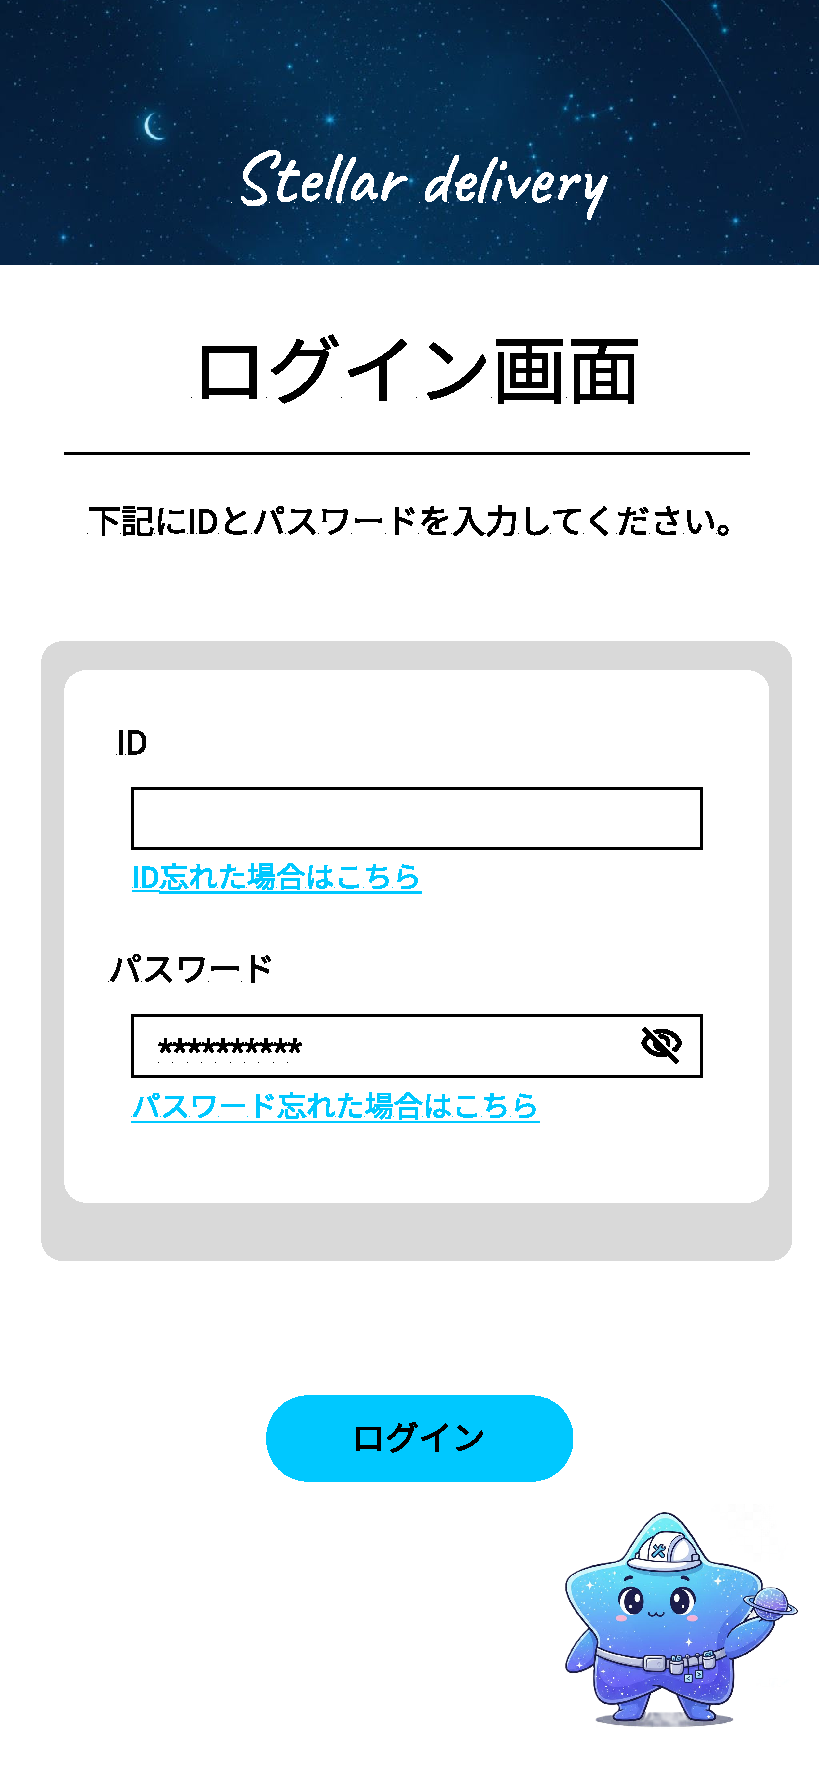
\includegraphics[width=0.75\textwidth]{./pic/Deliveryer画面デザイン/ログイン画面/ログイン画面.pdf}
  \caption{ログイン画面}
  \label{fig:ログイン画面}
\end{figure}

\subsubsection{パスワード確認・再設定画面}
図\ref{fig:パスワード確認・再設定画面}は、パスワード確認・再設定用URLをメールにて送信するための画面である。上記のログイン画面にてパスワードを忘れた際のリンクをクリックされた際に表示される画面である。ここでは利用者のアカウントのパスワード確認および再設定を行うためのメールを送ることで本アプリにログインできることを促す画面である。メールアドレスおよびIDを入力し、

図\ref{fig:パスワード確認メール送信画面}では、図\ref{fig:パスワード確認・再設定画面}にて送信ボタンを押すことで遷移される画面である。この画面では、メールアドレス宛にメールが送信されたことを利用者に伝える画面となってる。

\begin{figure}[tbp]
  \centering
  \begin{minipage}{.43\linewidth}
    \centering
    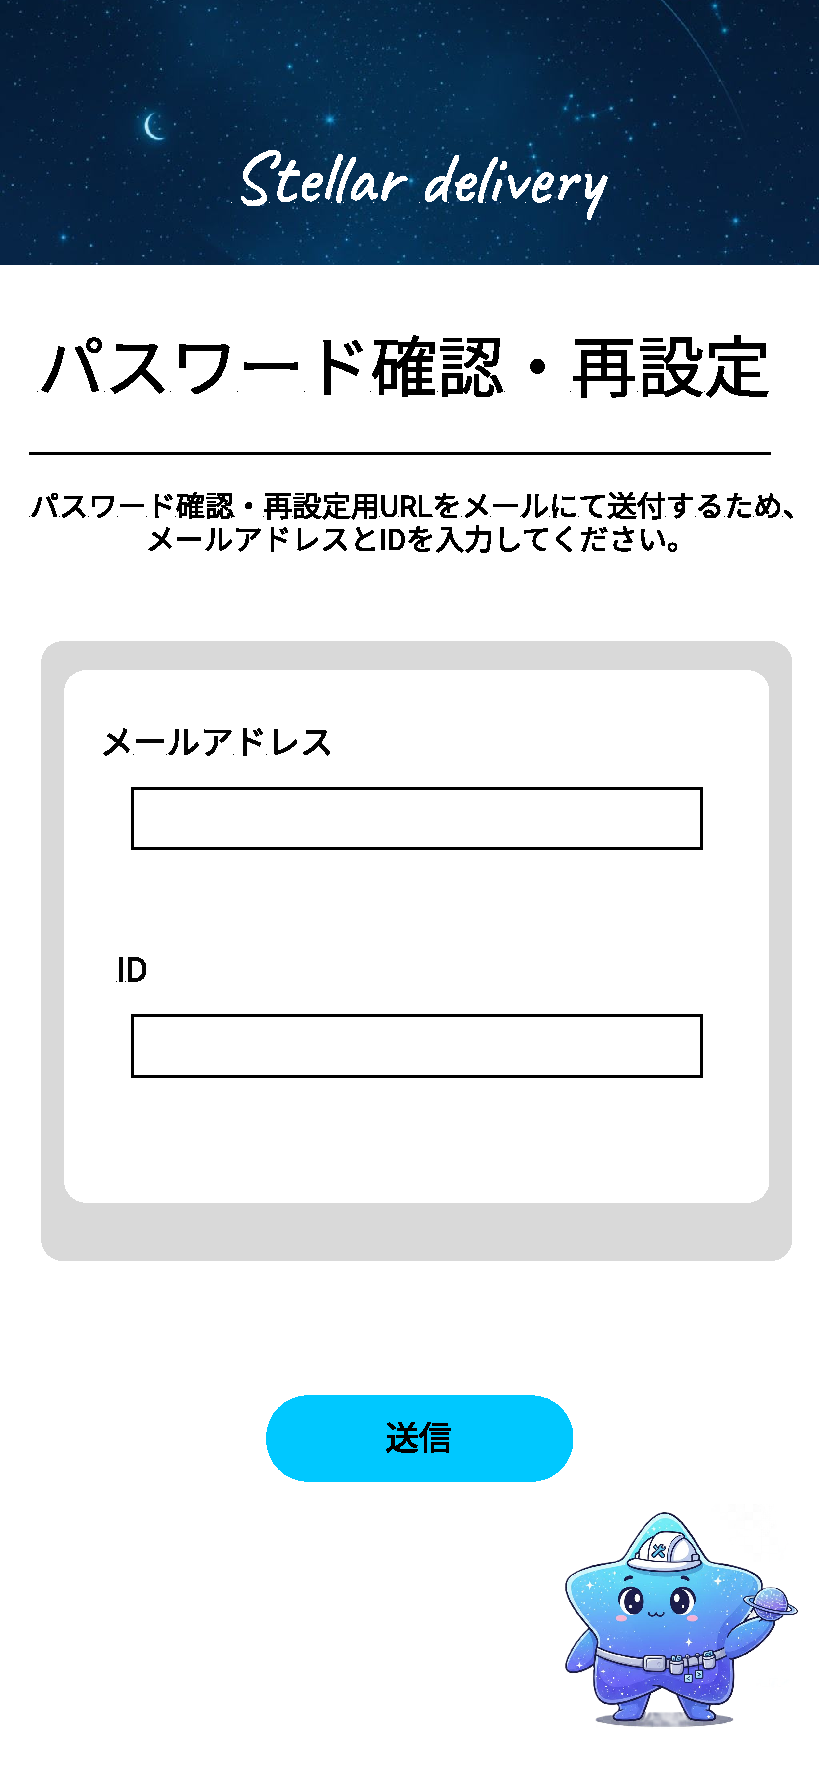
\includegraphics[width=\linewidth]{./pic/Deliveryer画面デザイン/ログイン画面/パスワード確認画面.pdf}
    \caption{パスワード確認・再設定画面}
    \label{fig:パスワード確認・再設定画面}
  \end{minipage}
  \hspace{5mm}
  \begin{minipage}{.43\linewidth}
    \centering
    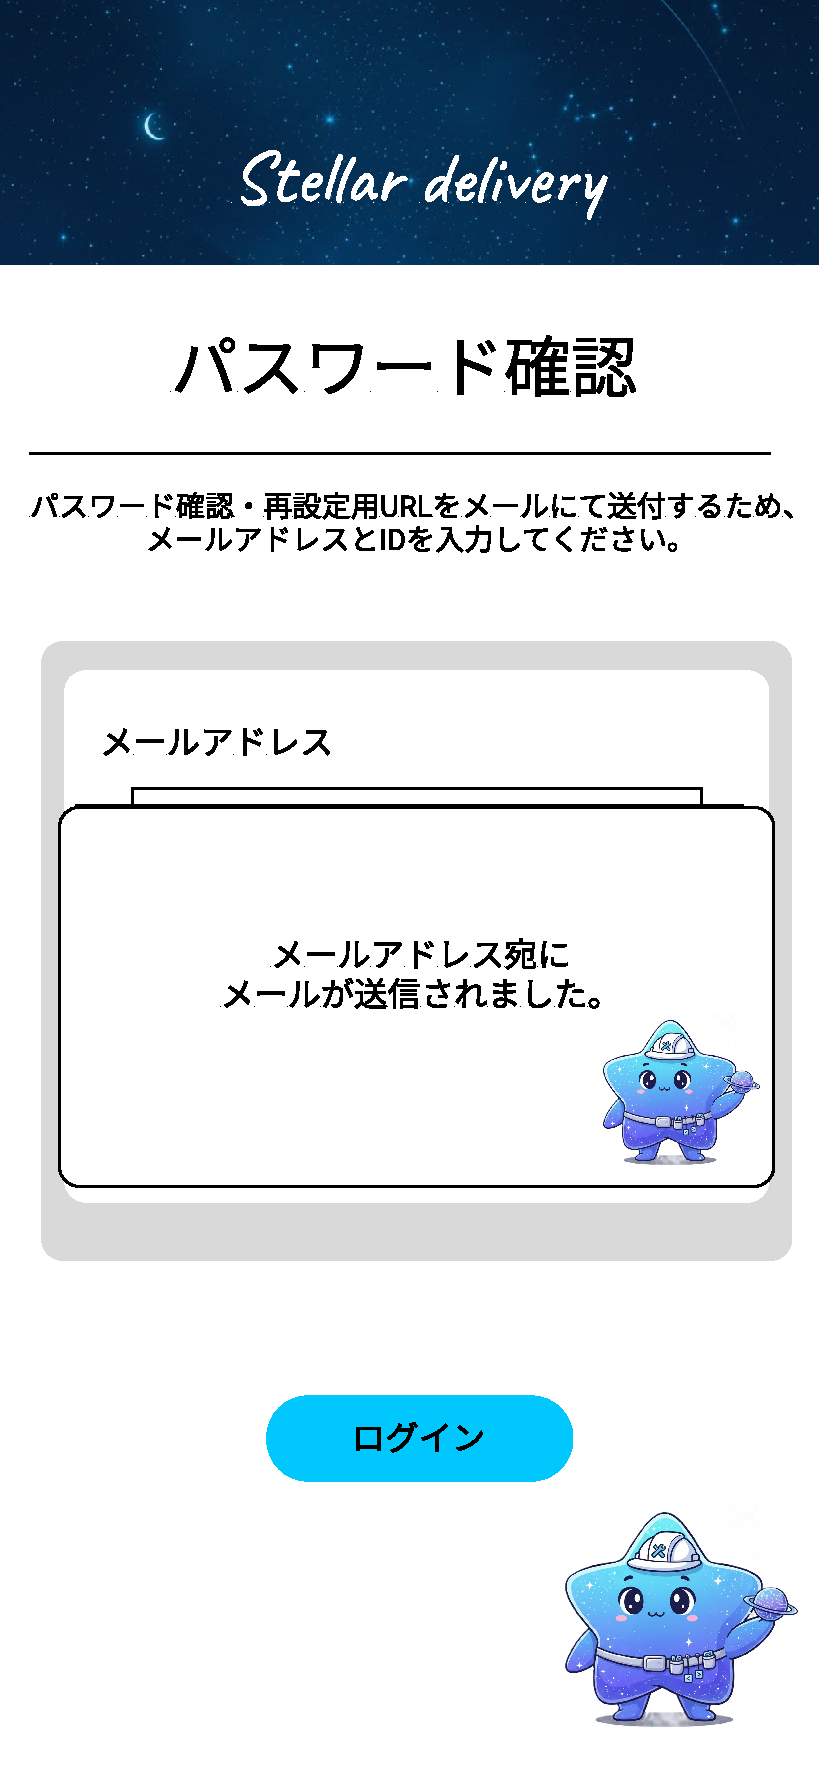
\includegraphics[width=\linewidth]{./pic/Deliveryer画面デザイン/ログイン画面/パスワード確認送信画面.pdf}
    \caption{パスワード確認メール送信画面}
    \label{fig:パスワード確認メール送信画面}
  \end{minipage}
\end{figure}

\subsubsection{ID確認画面}
図\ref{fig:ID確認画面}は、ID確認を行うためのURLをメールに送信する画面である。ここでは、利用者のメールアドレスおよびパスワードを入力し、ID確認用のメールを送ることで利用者がIDを確認しログイン処理が可能となる処置となっている。

図\ref{fig:ID確認送信画面}は、ID確認を行うためのURLをメールにて送信したことを知らせる画面である。

\begin{figure}[tbp]
  \centering
  \begin{minipage}{.43\linewidth}
    \centering
    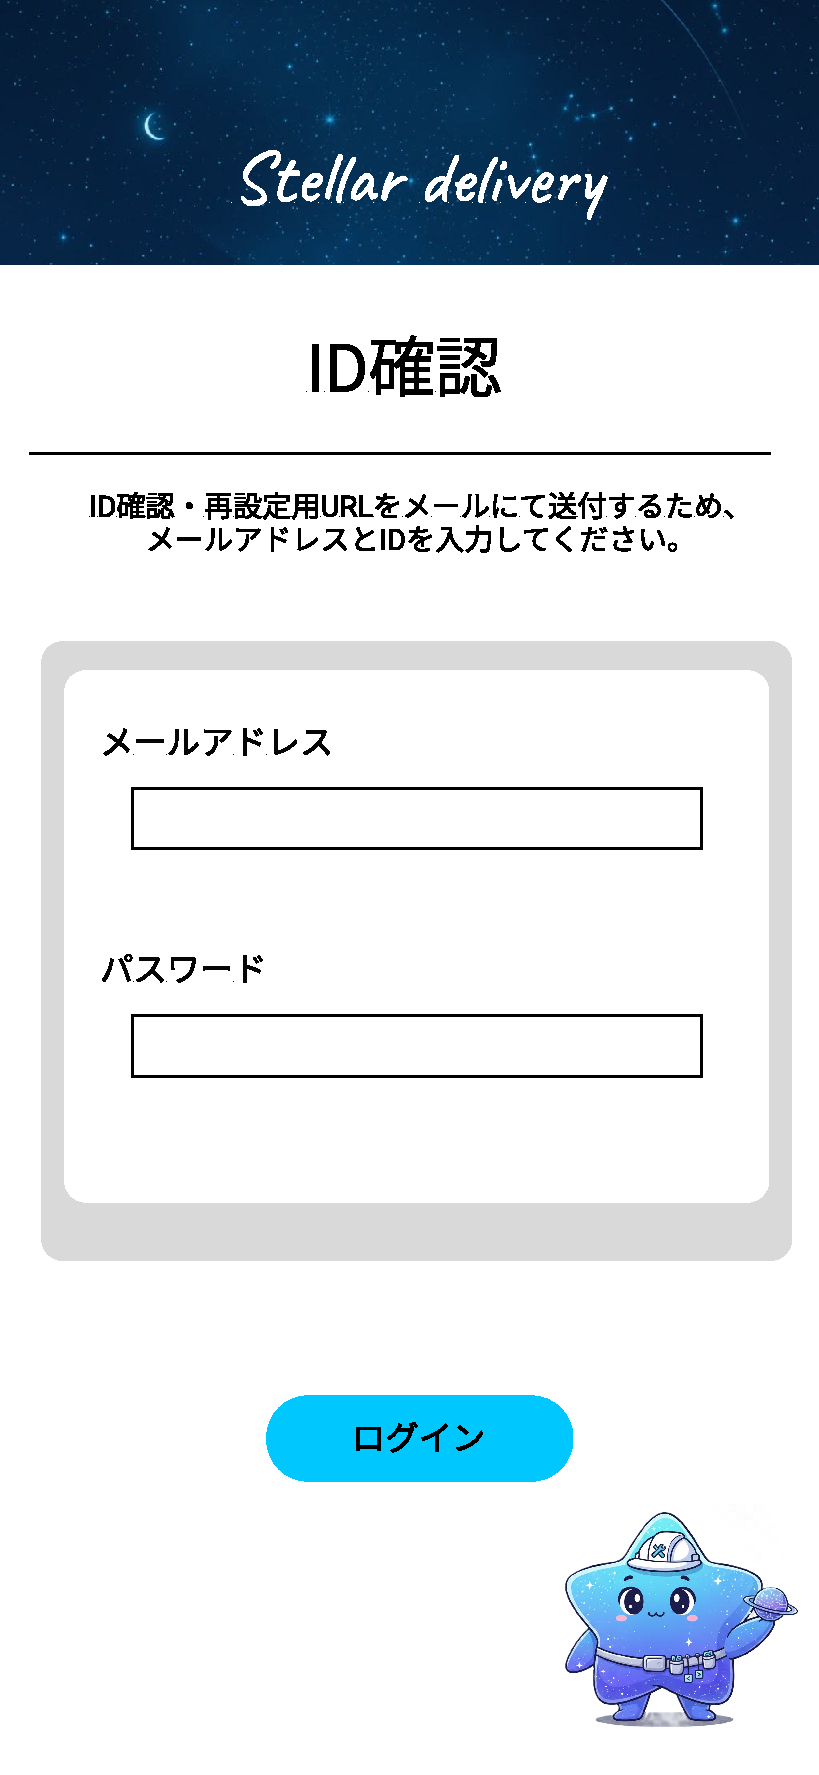
\includegraphics[width=\linewidth]{./pic/Deliveryer画面デザイン/ログイン画面/ID確認画面.pdf}
    \caption{ID確認画面}
    \label{fig:ID確認画面}
  \end{minipage}
  \hspace{5mm}
  \begin{minipage}{.43\linewidth}
    \centering
    \includegraphics[width=\linewidth]{./pic/Deliveryer画面デザイン/ログイン画面/ID確認送信画面.pdf}
    \caption{ID確認送信画面}
    \label{fig:ID確認送信画面}
  \end{minipage}
\end{figure}

\subsubsection{配達員側新規会員登録画面}
図\ref{fig:配達員側新規会員登録画面}では、図\ref{fig:ログイン画面}にて新規会員登録のリンクを選択することで表示される画面である。ここでは、まず利用手段について選択してもらう。利用手段に応じて登録する内容が変化する。図\ref{fig:配達員側新規会員登録画面2}では、入力内容の確認を行う画面である。

\begin{figure}[tbp]
  \centering
  \begin{minipage}{.43\linewidth}
    \centering
    \includegraphics[width=\linewidth]{./pic/Deliveryer画面デザイン/配達員側新規会員登録画面/新規会員登録.pdf}
    \caption{配達員側新規会員登録}
    \label{fig:配達員側新規会員登録}
  \end{minipage}
  \hspace{5mm}
  \begin{minipage}{.43\linewidth}
    \centering
    \includegraphics[width=\linewidth]{./pic/Deliveryer画面デザイン/配達員側新規会員登録画面/新規会員登録-1.pdf}
    \caption{配達員側新規会員確認画面}
    \label{fig:配達員側新規会員登録画面2}
  \end{minipage}
\end{figure}

そして、図\ref{fig:配達員側新規会員登録画面2}にて登録ボタンを押下することで図\ref{fig:配達員側新規会員登録画面3}に遷移する。図\ref{fig:配達員側新規会員登録画面3}では、新規会員登録完了を表示し、かつ配達員としてすぐに始めることができるよう履歴書入力を促すボタンが配置されている。ホームへというボタンを押下することで本アプリのホームに遷移される。


\begin{figure}[H]
  \centering
  \includegraphics[width=0.75\textwidth]{./pic/Deliveryer画面デザイン/配達員側新規会員登録画面/新規会員登録-2.pdf}
  \caption{配達員側新規会員登録完了画面}
  \label{fig:配達員側新規会員登録画面3}
\end{figure}

\subsubsection{ホーム画面}
図\ref{fig:ホーム画面}では、本アプリをログインした際にホーム画面として表示される画面である。本アプリでは、フッターにて求人検索、マップ、受注、マイページ、ホームのボタンがあり、常にそれぞれの画面に遷移することが可能である。

図\ref{fig:ホーム画面}には、キーワードにて求人検索ができる検索バーと求人情報おすすめを表示する機能がある。また、配達中であれば受注した依頼の中で直近の配達内容を表示する機能がある。ここでは、ルート確認や配達完了、配達状況を確認することができ、アプリを開いた際にすぐに情報が確認できるものとなっている。


\begin{figure}[H]
  \centering
  \includegraphics[width=0.75\textwidth]{./pic/Deliveryer画面デザイン/ホーム画面.pdf}
  \caption{ホーム画面}
  \label{fig:ホーム画面}
\end{figure}

\subsubsection{求人検索画面}
図\ref{fig:求人検索画面}では、求人検索を行うための画面である。ここで求人の一覧を確認することができ、地域や商品数、そして届ける手段としておすすめだと考えられる求人を表示する機能がある。


\begin{figure}[H]
  \centering
  \includegraphics[width=0.75\textwidth]{./pic/Deliveryer画面デザイン/求人検索画面/求人検索画面.pdf}
  \caption{求人検索画面}
  \label{fig:求人検索画面}
\end{figure}

図\ref{fig:求人検索詳細画面}では、図\ref{fig:求人検索画面}にてピックアップされた内容をタップすることで表示される画面である。この画面では、求人詳細を示しており、注文内容や目安の距離、報酬金額が一覧にて確認することができる。また、下記にあるルート表示ボタンを押下することで図\ref{fig:求人ルート表示画面}のような求人ルートがマップの形で確認できる画面に遷移することが可能である。

\begin{figure}[tbp]
  \centering
  \begin{minipage}{.43\linewidth}
    \centering
    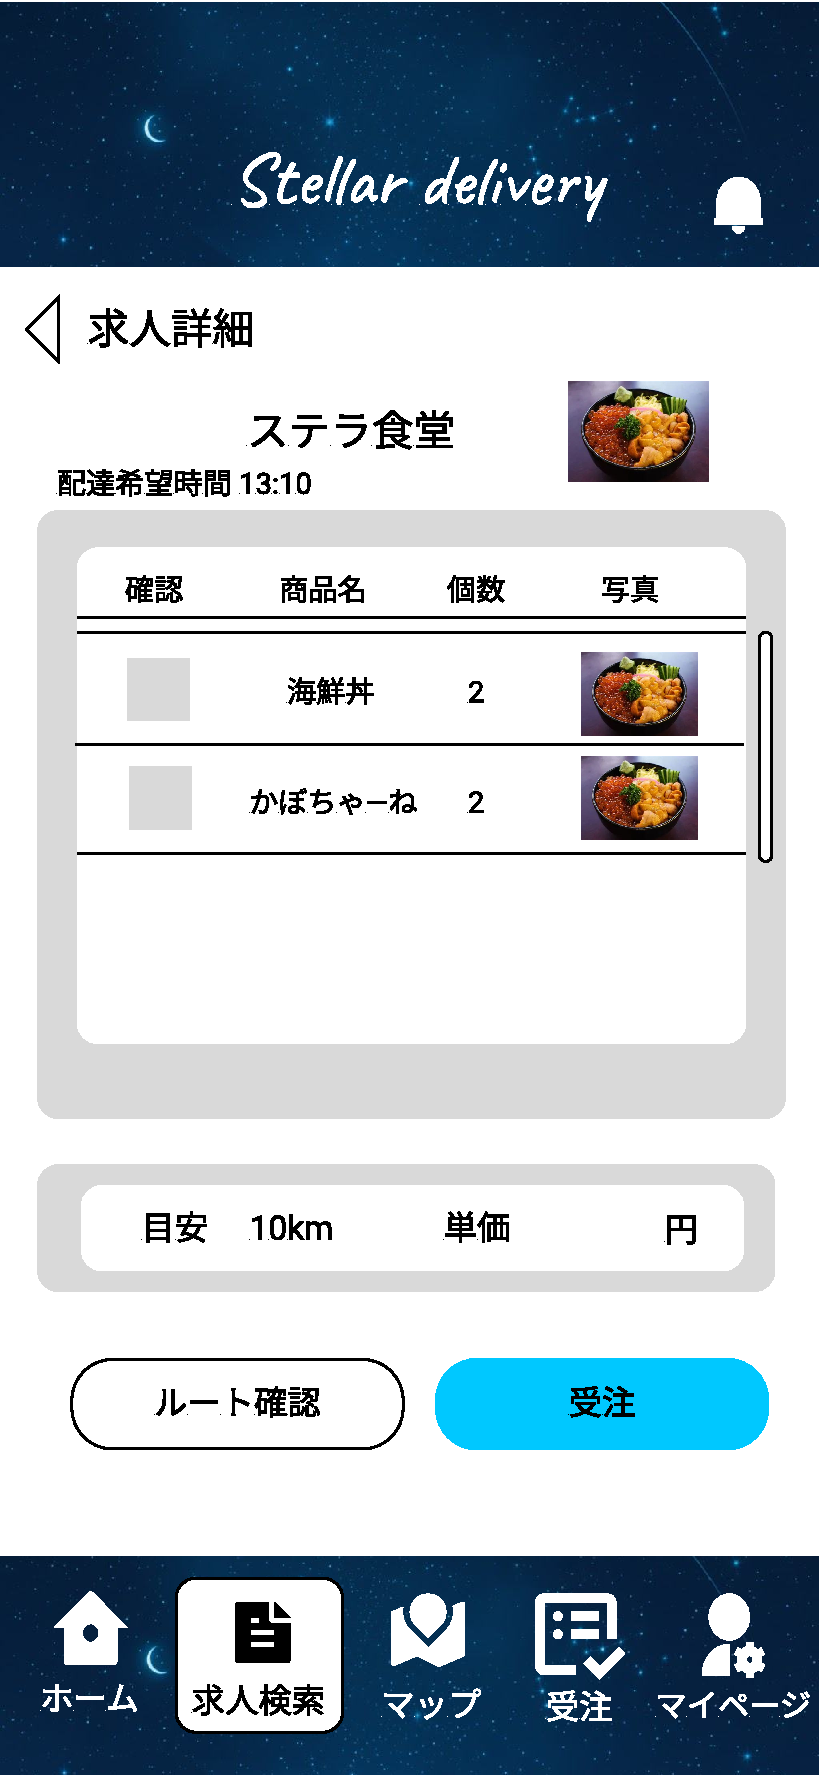
\includegraphics[width=\linewidth]{./pic/Deliveryer画面デザイン/求人検索画面/求人検索内容確認.pdf}
    \caption{求人検索詳細画面}
    \label{fig:求人検索詳細画面}
  \end{minipage}
  \hspace{5mm}
  \begin{minipage}{.43\linewidth}
    \centering
    \includegraphics[width=\linewidth]{./pic/Deliveryer画面デザイン/求人検索画面/求人ルート表示画面.pdf}
    \caption{求人ルート表示画面}
    \label{fig:求人ルート表示画面}
  \end{minipage}
\end{figure}

%求人確定画面をかく

\subsubsection{マップ機能}
図\ref{fig:配達先住所検索画面}では、マップにて求人情報および配達先が確認できる画面である。ここにおいて、店舗はジャンルによってアイコンが異なり、配達先を赤い旗マークとしている。また、求人一覧を下部にて確認することができ、求人内容の検索を利用することも可能な画面である。

図\ref{fig:求人ルート表示画面}では、図\ref{fig:配達先住所検索画面}にて押下された求人内容の距離をマップにて視覚的に目的地を表示する画面である。

\begin{figure}[tbp]
  \centering
  \begin{minipage}{.43\linewidth}
    \centering
    \includegraphics[width=\linewidth]{./pic/Deliveryer画面デザイン/マップ画面/配達先住所検索画面.pdf}
    \caption{配達先住所検索画面}
    \label{fig:配達先住所検索画面}
  \end{minipage}
  \hspace{5mm}
  \begin{minipage}{.43\linewidth}
    \centering
    \includegraphics[width=\linewidth]{./pic/Deliveryer画面デザイン/マップ画面/求人ルート表示画面.pdf}
    \caption{求人ルート表示画面}
    \label{fig:求人ルート表示画面}
  \end{minipage}
\end{figure}

図\ref{fig:求人受注画面}では、前述の図\ref{fig:求人検索詳細画面}と同様の機能を有している画面である。


\begin{figure}[H]
  \centering
  \includegraphics[width=0.75\textwidth]{./pic/Deliveryer画面デザイン/マップ画面/求人受注画面.pdf}
  \caption{求人受注画面}
  \label{fig:求人受注画面}
\end{figure}

\subsubsection{受注一覧画面}
図\ref{fig:受注依頼一覧画面}では、受注した依頼の一覧を表示する画面である。受注依頼は最大3つまでであり、それぞれの受注依頼に対して配達希望時間や現在時刻から何分後なのかが表示される。

\begin{figure}[H]
  \centering
  \includegraphics[width=0.75\textwidth]{./pic/Deliveryer画面デザイン/受注依頼一覧画面/求人受注画面.pdf}
  \caption{求人受注画面}
  \label{fig:求人受注画面}
\end{figure}

図\ref{fig:依頼詳細画面}では、受注内容を各因子、配達完了やルート確認を行う画面である。

\begin{figure}[H]
  \centering
  \includegraphics[width=0.75\textwidth]{./pic/Deliveryer画面デザイン/受注依頼一覧画面/依頼詳細画面.pdf}
  \caption{依頼詳細画面}
  \label{fig:依頼詳細画面}
\end{figure}

\subsubsection{通知画面}
図\ref{fig:配達業務通知画面}では、通知を行う画面である。ここでは配達業務および運営メールの切り替えを行うことができ、配達業務では配達完了メールなどが届けられる。

図\ref{fig:メール詳細画面}では、図\ref{fig:配達業務通知画面}にて選択したメールの詳細を見ることができる画面である。

\begin{figure}[tbp]
  \centering
  \begin{minipage}{.43\linewidth}
    \centering
    \includegraphics[width=\linewidth]{./pic/Deliveryer画面デザイン/通知画面/通知画面.pdf}
    \caption{配達業務通知画面}
    \label{fig:配達業務通知画面}
  \end{minipage}
  \hspace{5mm}
  \begin{minipage}{.43\linewidth}
    \centering
    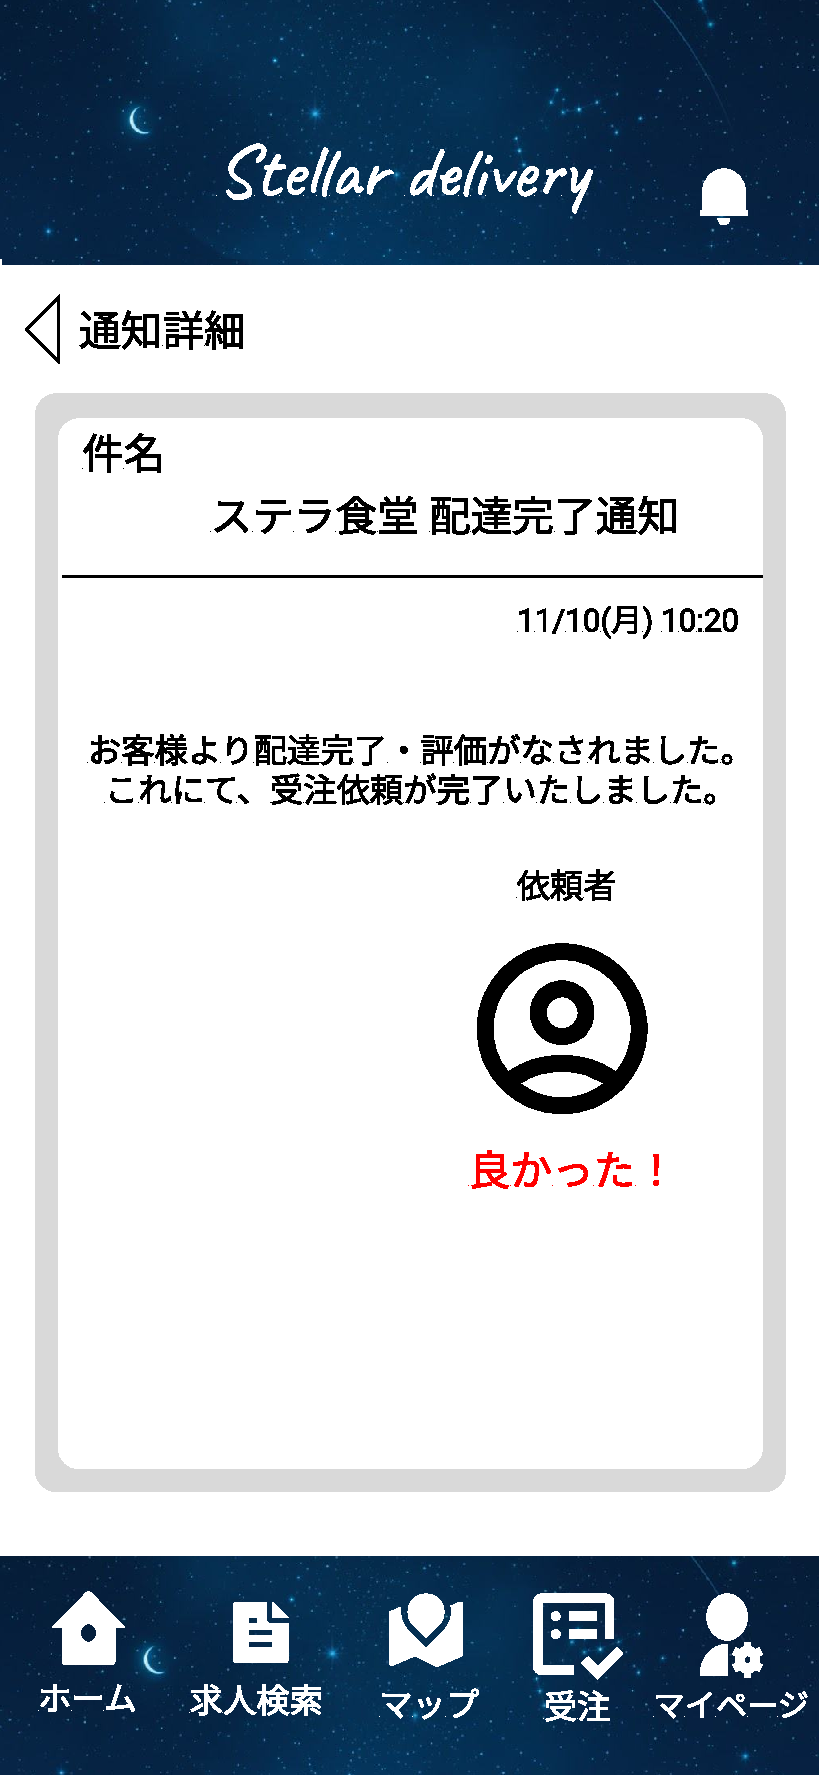
\includegraphics[width=\linewidth]{./pic/Deliveryer画面デザイン/通知画面/メール詳細画面.pdf}
    \caption{配達業務通知詳細画面}
    \label{fig:メール詳細画面}
  \end{minipage}
\end{figure}

図\ref{fig:運営通知画面}では、図\ref{fig:配達業務通知画面}にて切り替えた運営メールを一覧を表示する画面である。そして、図\ref{fig:メール詳細2}では前述と同様にメールの詳細が確認できる画面である。

%運営通知画面のファイル名を変更する。

\begin{figure}[tbp]
  \centering
  \begin{minipage}{.43\linewidth}
    \centering
    \includegraphics[width=\linewidth]{./pic/Deliveryer画面デザイン/通知画面/通知画面_運営メール.pdf}
    \caption{運営通知画面}
    \label{fig:運営通知画面}
  \end{minipage}
  \hspace{5mm}
  \begin{minipage}{.43\linewidth}
    \centering
    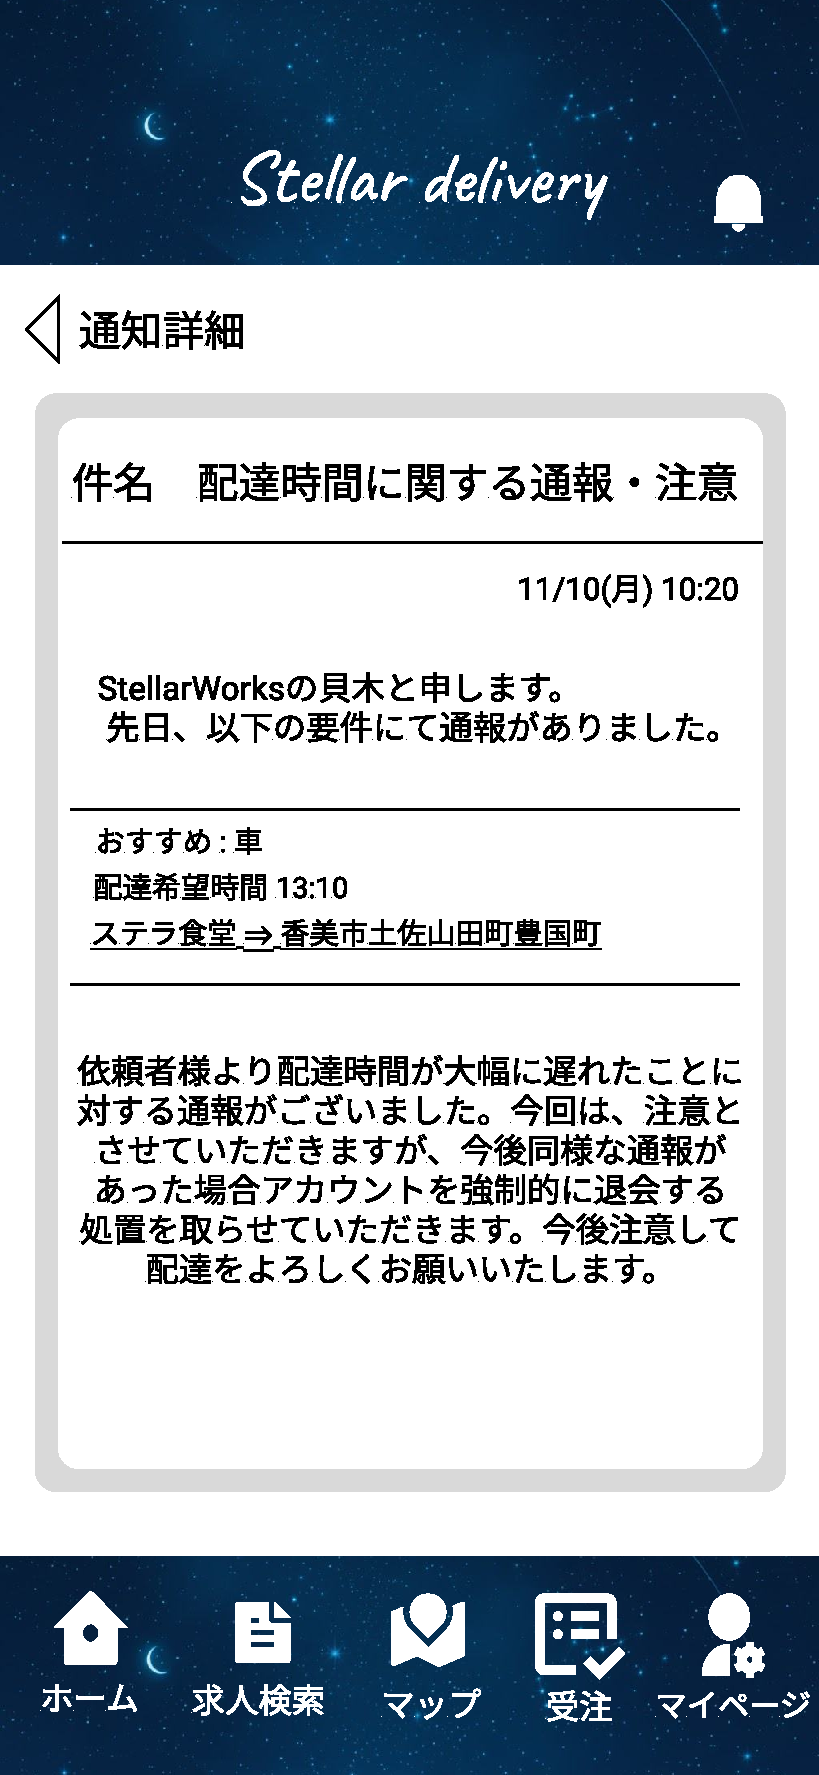
\includegraphics[width=\linewidth]{./pic/Deliveryer画面デザイン/通知画面/メール詳細画面-1.pdf}
    \caption{運営メール詳細画面}
    \label{fig:メール詳細2}
  \end{minipage}
\end{figure}

\subsubsection{マイページ}
図\ref{fig:マイページ}では、会員登録、履歴書、配達履歴、パスワード確認、口座情報管理、給与明細、運営問い合わせ、設定、ログアウト・退会を行う画面である。主に自身のアカウントに関する設定の変更などを行うことができる。

%マイページの図を貼り着ける

\subsubsection{会員情報}

\subsection{店舗側}
\subsubsection{業務画面}
\begin{figure}[H]
  \centering
  \includegraphics[width=0.75\textwidth]{./pic/store画面デザイン/業務画面.pdf}
  \caption{業務画面}
  \label{fig:業務画面}
\end{figure}

\subsubsection{メニュー情報変更選択画面}
\begin{figure}[H]
  \centering
  \includegraphics[width=0.75\textwidth]{./pic/store画面デザイン/メニュー情報変更画面.pdf}
  \caption{メニュー情報変更選択画面}
  \label{fig:メニュー情報変更選択画面}
\end{figure}

\subsubsection{メニュー情報登録画面}
\begin{figure}[H]
  \centering
  \includegraphics[width=0.75\textwidth]{./pic/store画面デザイン/メニュー情報登録画面.pdf}
  \caption{メニュー情報登録画面}
  \label{fig:メニュー情報登録画面}
\end{figure}

\subsubsection{メニュー情報削除画面}
\begin{figure}[H]
  \centering
  \includegraphics[width=0.75\textwidth]{./pic/store画面デザイン/メニュー情報削除画面.pdf}
  \caption{メニュー情報削除画面}
  \label{fig:メニュー情報削除画面}
\end{figure}

\subsubsection{メニュー情報変更画面}
\begin{figure}[H]
  \centering
  \includegraphics[width=0.75\textwidth]{./pic/store画面デザイン/メニュー情報変更画面-1.pdf}
  \caption{メニュー情報変更画面}
  \label{fig:メニュー情報変更画面}
\end{figure}

\subsubsection{在庫ステータス変更画面}
\begin{figure}[H]
  \centering
  \includegraphics[width=0.75\textwidth]{./pic/store画面デザイン/在庫ステータス変更画面}
  \caption{在庫ステータス変更画面}
  \label{fig:在庫ステータス変更画面}
\end{figure}

\subsubsection{注文管理画面}
\begin{figure}[H]
  \centering
  \includegraphics[width=0.75\textwidth]{./pic/store画面デザイン/注文管理画面.pdf}
  \caption{注文管理画面}
  \label{fig:注文管理画面}
\end{figure}

\subsubsection{受注一覧画面}
\begin{figure}[H]
  \centering
  \includegraphics[width=0.75\textwidth]{./pic/store画面デザイン/受注一覧画面.pdf}
  \caption{受注一覧画面}
  \label{fig:受注一覧画面}
\end{figure}

\subsubsection{配達員情報確認画面}
\begin{figure}[H]
  \centering
  \includegraphics[width=0.75\textwidth]{./pic/store画面デザイン/配達員情報確認画面.pdf}
  \caption{配達員情報確認画面}
  \label{fig:配達員情報確認画面}
\end{figure}

\subsubsection{受け渡し完了確認画面}
\begin{figure}[H]
  \centering
  \includegraphics[width=0.75\textwidth]{./pic/store画面デザイン/受け渡し完了確認画面.pdf}
  \caption{受け渡し完了確認画面}
  \label{fig:受け渡し完了確認画面}
\end{figure}

\subsubsection{配達トラブル報告画面}
\begin{figure}[H]
  \centering
  \includegraphics[width=0.75\textwidth]{./pic/store画面デザイン/配達トラブル報告画面.pdf}
  \caption{配達トラブル報告画面}
  \label{fig:配達トラブル報告画面}
\end{figure}

\subsubsection{売上画面}
\begin{figure}[H]
  \centering
  \includegraphics[width=0.75\textwidth]{./pic/store画面デザイン/売上画面.pdf}
  \caption{売上画面}
  \label{fig:売上画面}
\end{figure}

\subsubsection{明細表示画面}
\begin{figure}[H]
  \centering
  \includegraphics[width=0.75\textwidth]{./pic/store画面デザイン/明細表示画面.pdf}
  \caption{明細表示画面}
  \label{fig:明細表示画面}
\end{figure}

\subsubsection{マイページ}
\begin{figure}[H]
  \centering
  \includegraphics[width=0.75\textwidth]{./pic/store画面デザイン/マイページ.pdf}
  \caption{マイページ}
  \label{fig:マイページ}
\end{figure}

\subsubsection{店舗情報確認・編集画面}
\begin{figure}[H]
  \centering
  \includegraphics[width=0.75\textwidth]{./pic/store画面デザイン/店舗情報確認・編集画面.pdf}
  \caption{店舗情報確認・編集画面}
  \label{fig:店舗情報確認・編集画面}
\end{figure}

\subsubsection{許可書ファイルアップロード画面}
\begin{figure}[H]
  \centering
  \includegraphics[width=0.75\textwidth]{./pic/store画面デザイン/許可書ファイルアップロード.pdf}
  \caption{許可書ファイルアップロード画面}
  \label{fig:許可書ファイルアップロード画面}
\end{figure}

\subsubsection{パスワード変更画面}
\begin{figure}[H]
  \centering
  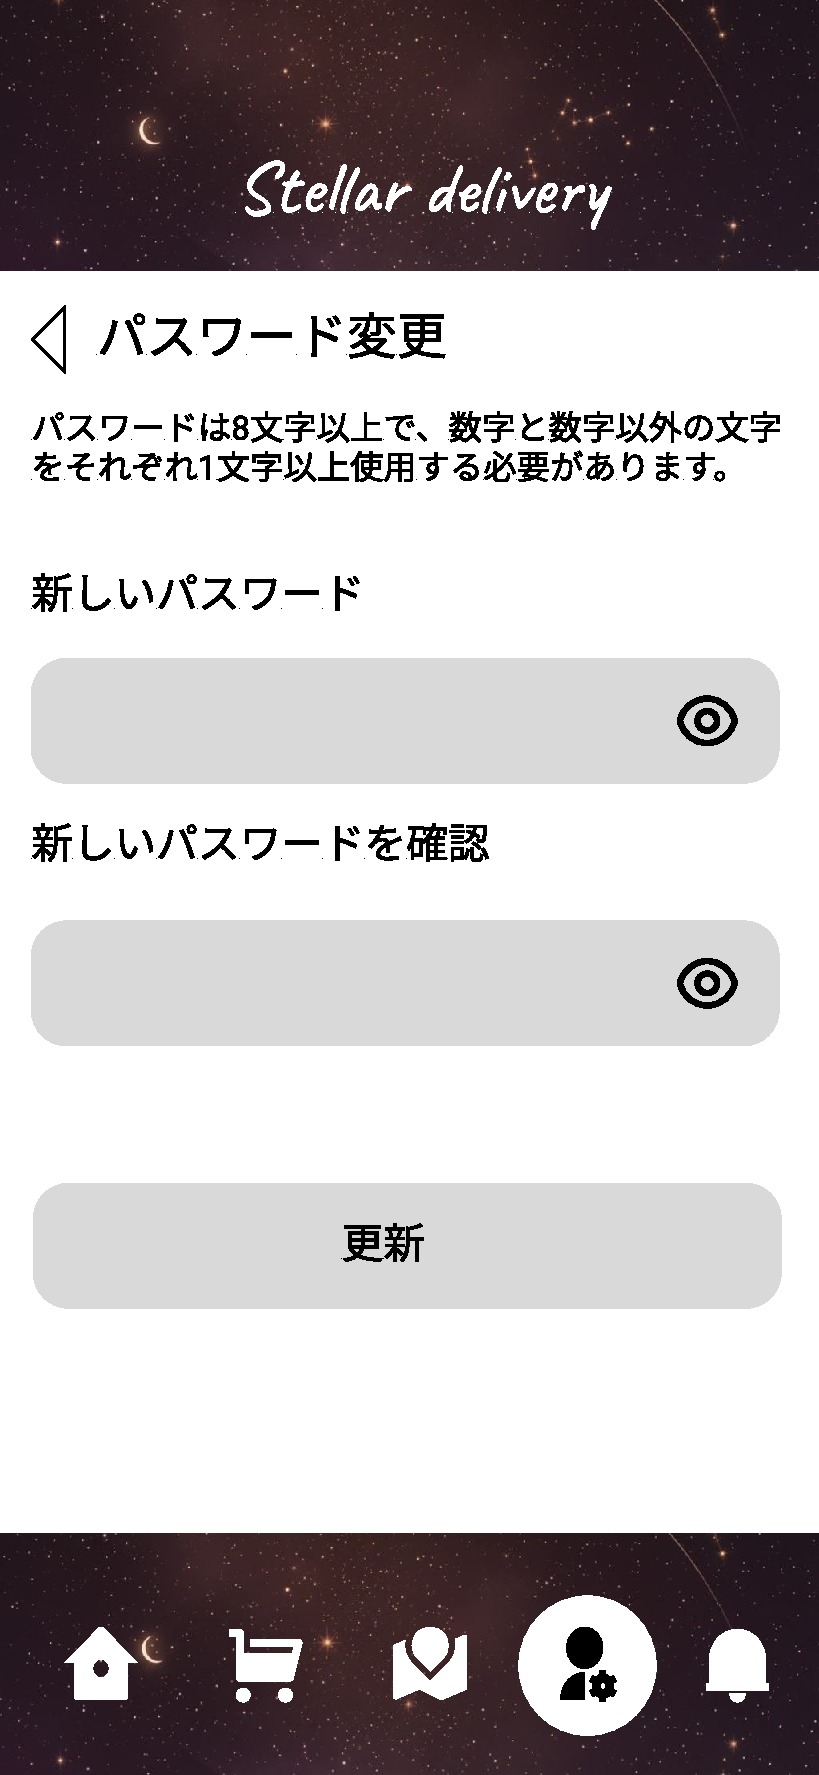
\includegraphics[width=0.75\textwidth]{./pic/store画面デザイン/パスワード変更画面.pdf}
  \caption{パスワード変更画面}
  \label{fig:パスワード変更画面}
\end{figure}

\subsubsection{口座情報登録・確認画面}
\begin{figure}[H]
  \centering
  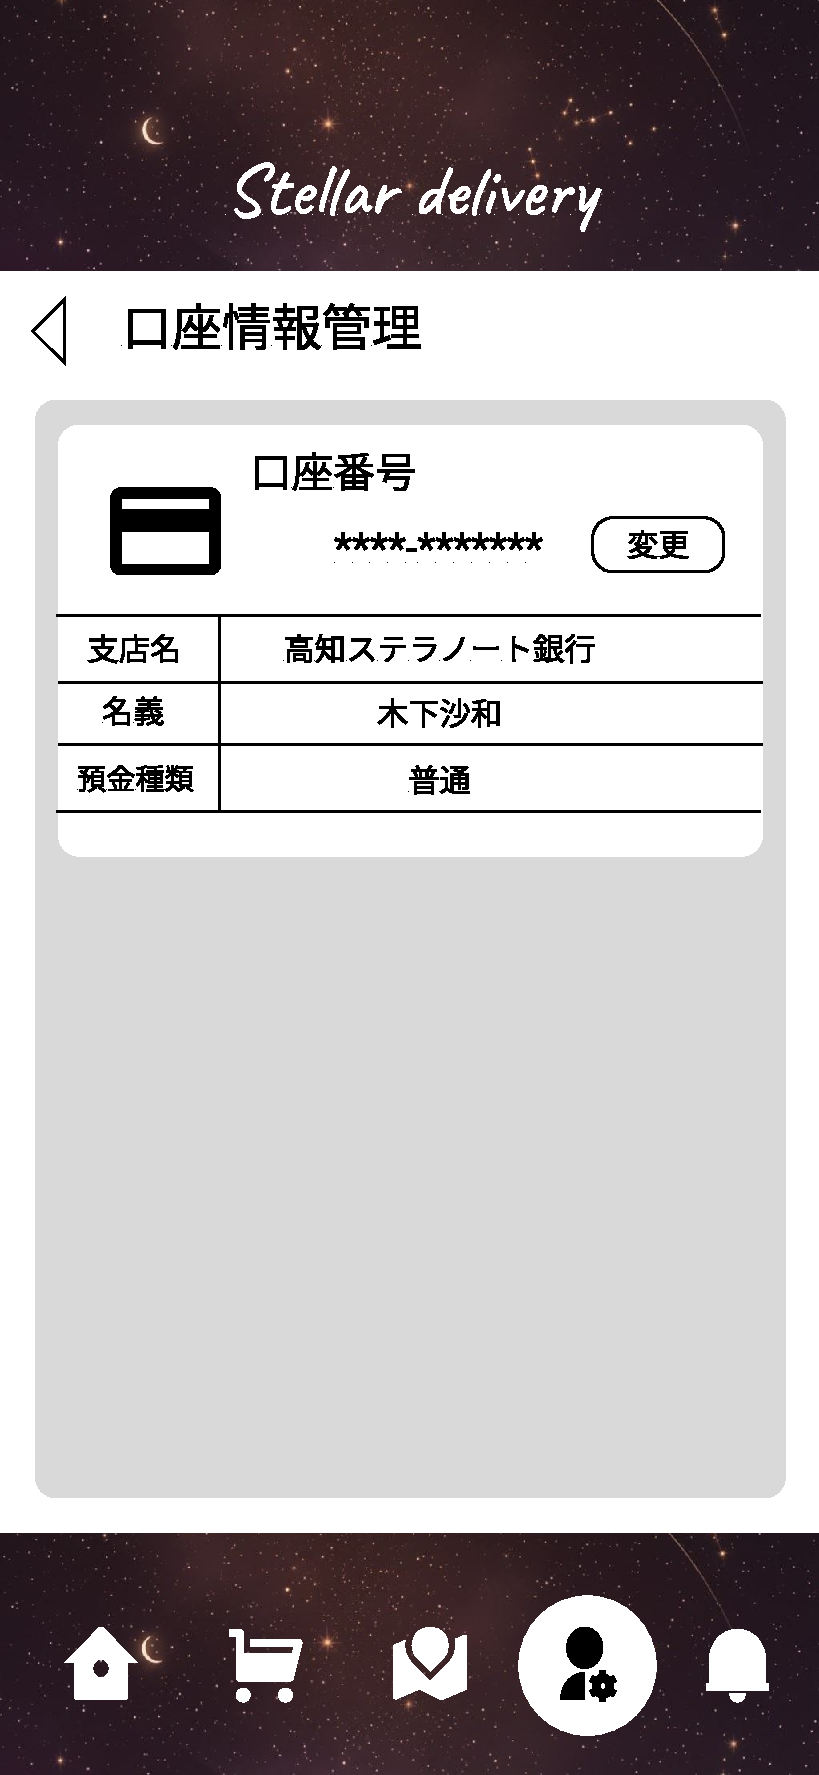
\includegraphics[width=0.75\textwidth]{./pic/store画面デザイン/口座情報登録・確認画面.pdf}
  \caption{口座情報登録・確認画面}
  \label{fig:口座情報登録・確認画面}
\end{figure}

\subsubsection{問い合わせ画面}
\begin{figure}[H]
  \centering
  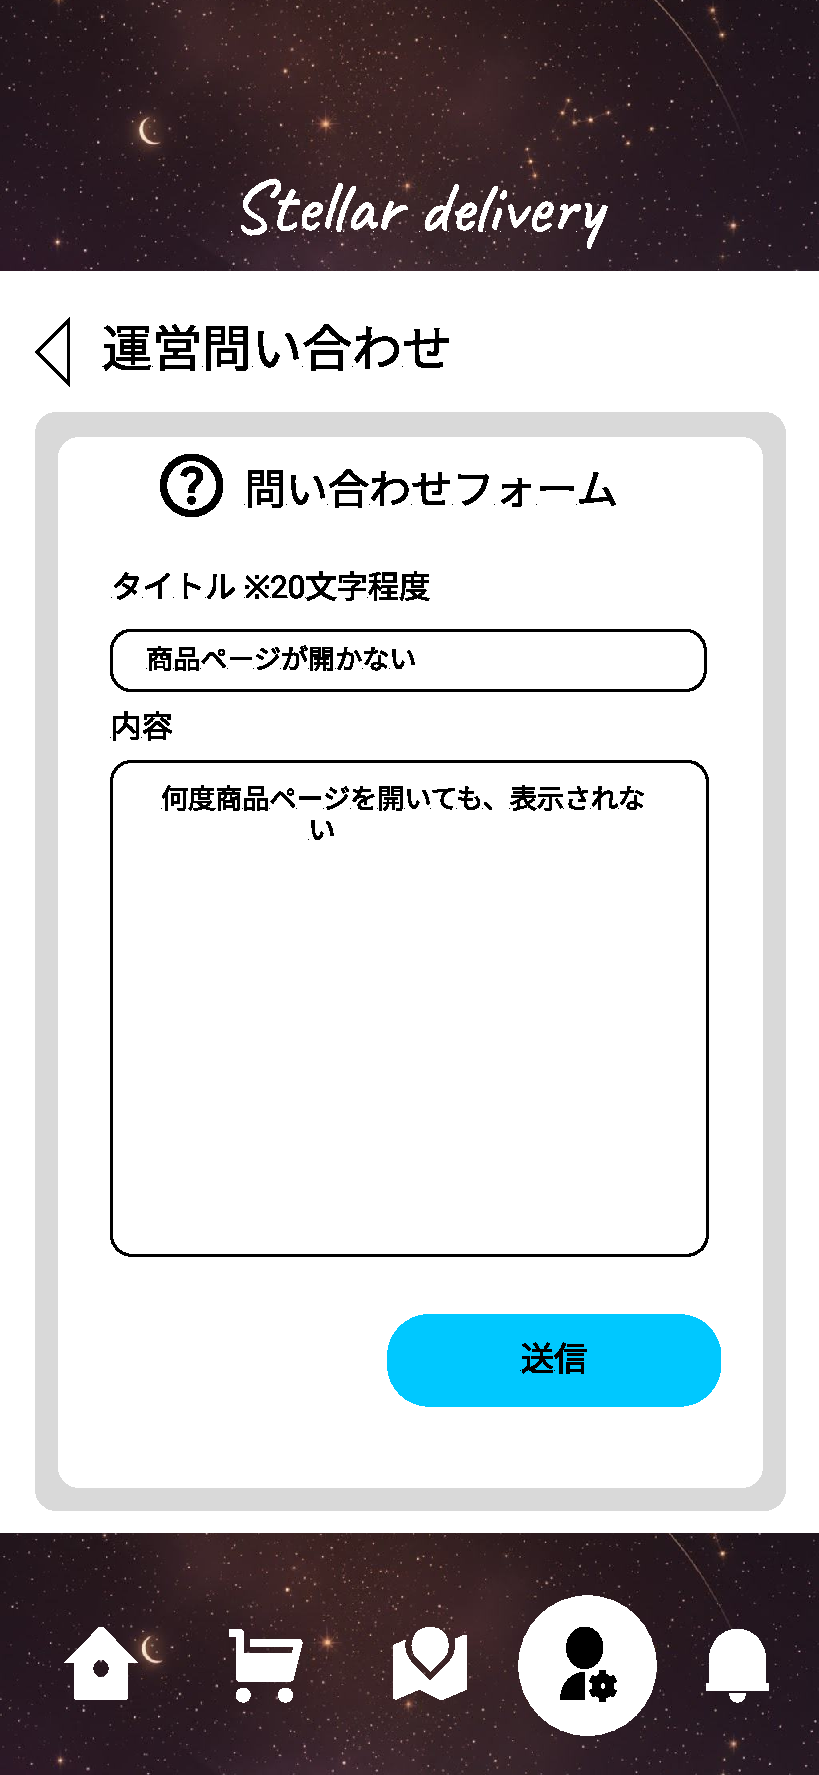
\includegraphics[width=0.75\textwidth]{./pic/store画面デザイン/問い合わせ画面.pdf}
  \caption{問い合わせ画面}
  \label{fig:問い合わせ画面}
\end{figure}

\subsubsection{ログアウト・退会画面}
\begin{figure}[H]
  \centering
  \includegraphics[width=0.75\textwidth]{./pic/store画面デザイン/ログアウト・退会画面.pdf}
  \caption{ログアウト・退会画面}
  \label{fig:ログアウト・退会画面}
\end{figure}

\subsubsection{通知画面}
\begin{figure}[H]
  \centering
  \includegraphics[width=0.75\textwidth]{./pic/store画面デザイン/通知画面.pdf}
  \caption{通知画面}
  \label{fig:通知画面}
\end{figure}



\subsection{管理者側}
ここでは管理者側の画面について説明する。

\subsubsection{管理者用端末アプリ起動画面/ログイン画面}
図\ref{fig:管理者用端末アプリ起動画面}、図\ref{fig:ログイン画面}は管理者用端末のアプリ起動画面およびログイン画面である。
管理者は管理者IDとパスワードでログインする。
管理者IDを忘れた場合は、図\ref{fig:管理者IDを忘れた場合}でメールアドレスとパスワードを入力し、メールにて送付されたURLを開くことで、
図\ref{fig:管理者ID確認画面}から管理者IDを確認することができる。
パスワードを忘れた場合は、図\ref{fig:パスワードを忘れた場合}で管理者IDとメールアドレスを入力し、メールにて送付されたURLを開くことで、
図\ref{fig:パスワード再設定画面}からパスワードの再設定を行うことができる。
\begin{figure}[H]
  \centering
  \includegraphics[width=0.75\textwidth]{./pic/administrator画面デザイン/0_ログイン/0_管理者用端末_アプリ起動画面.pdf}
  \caption{管理者用端末アプリ起動画面}
  \label{fig:管理者用端末アプリ起動画面}
\end{figure}
\begin{figure}[H]
  \centering
  \includegraphics[width=0.75\textwidth]{./pic/administrator画面デザイン/0_ログイン/01_ログイン画面.pdf}
  \caption{ログイン画面}
  \label{fig:ログイン画面}
\end{figure}

\begin{figure}[H]
  \centering
  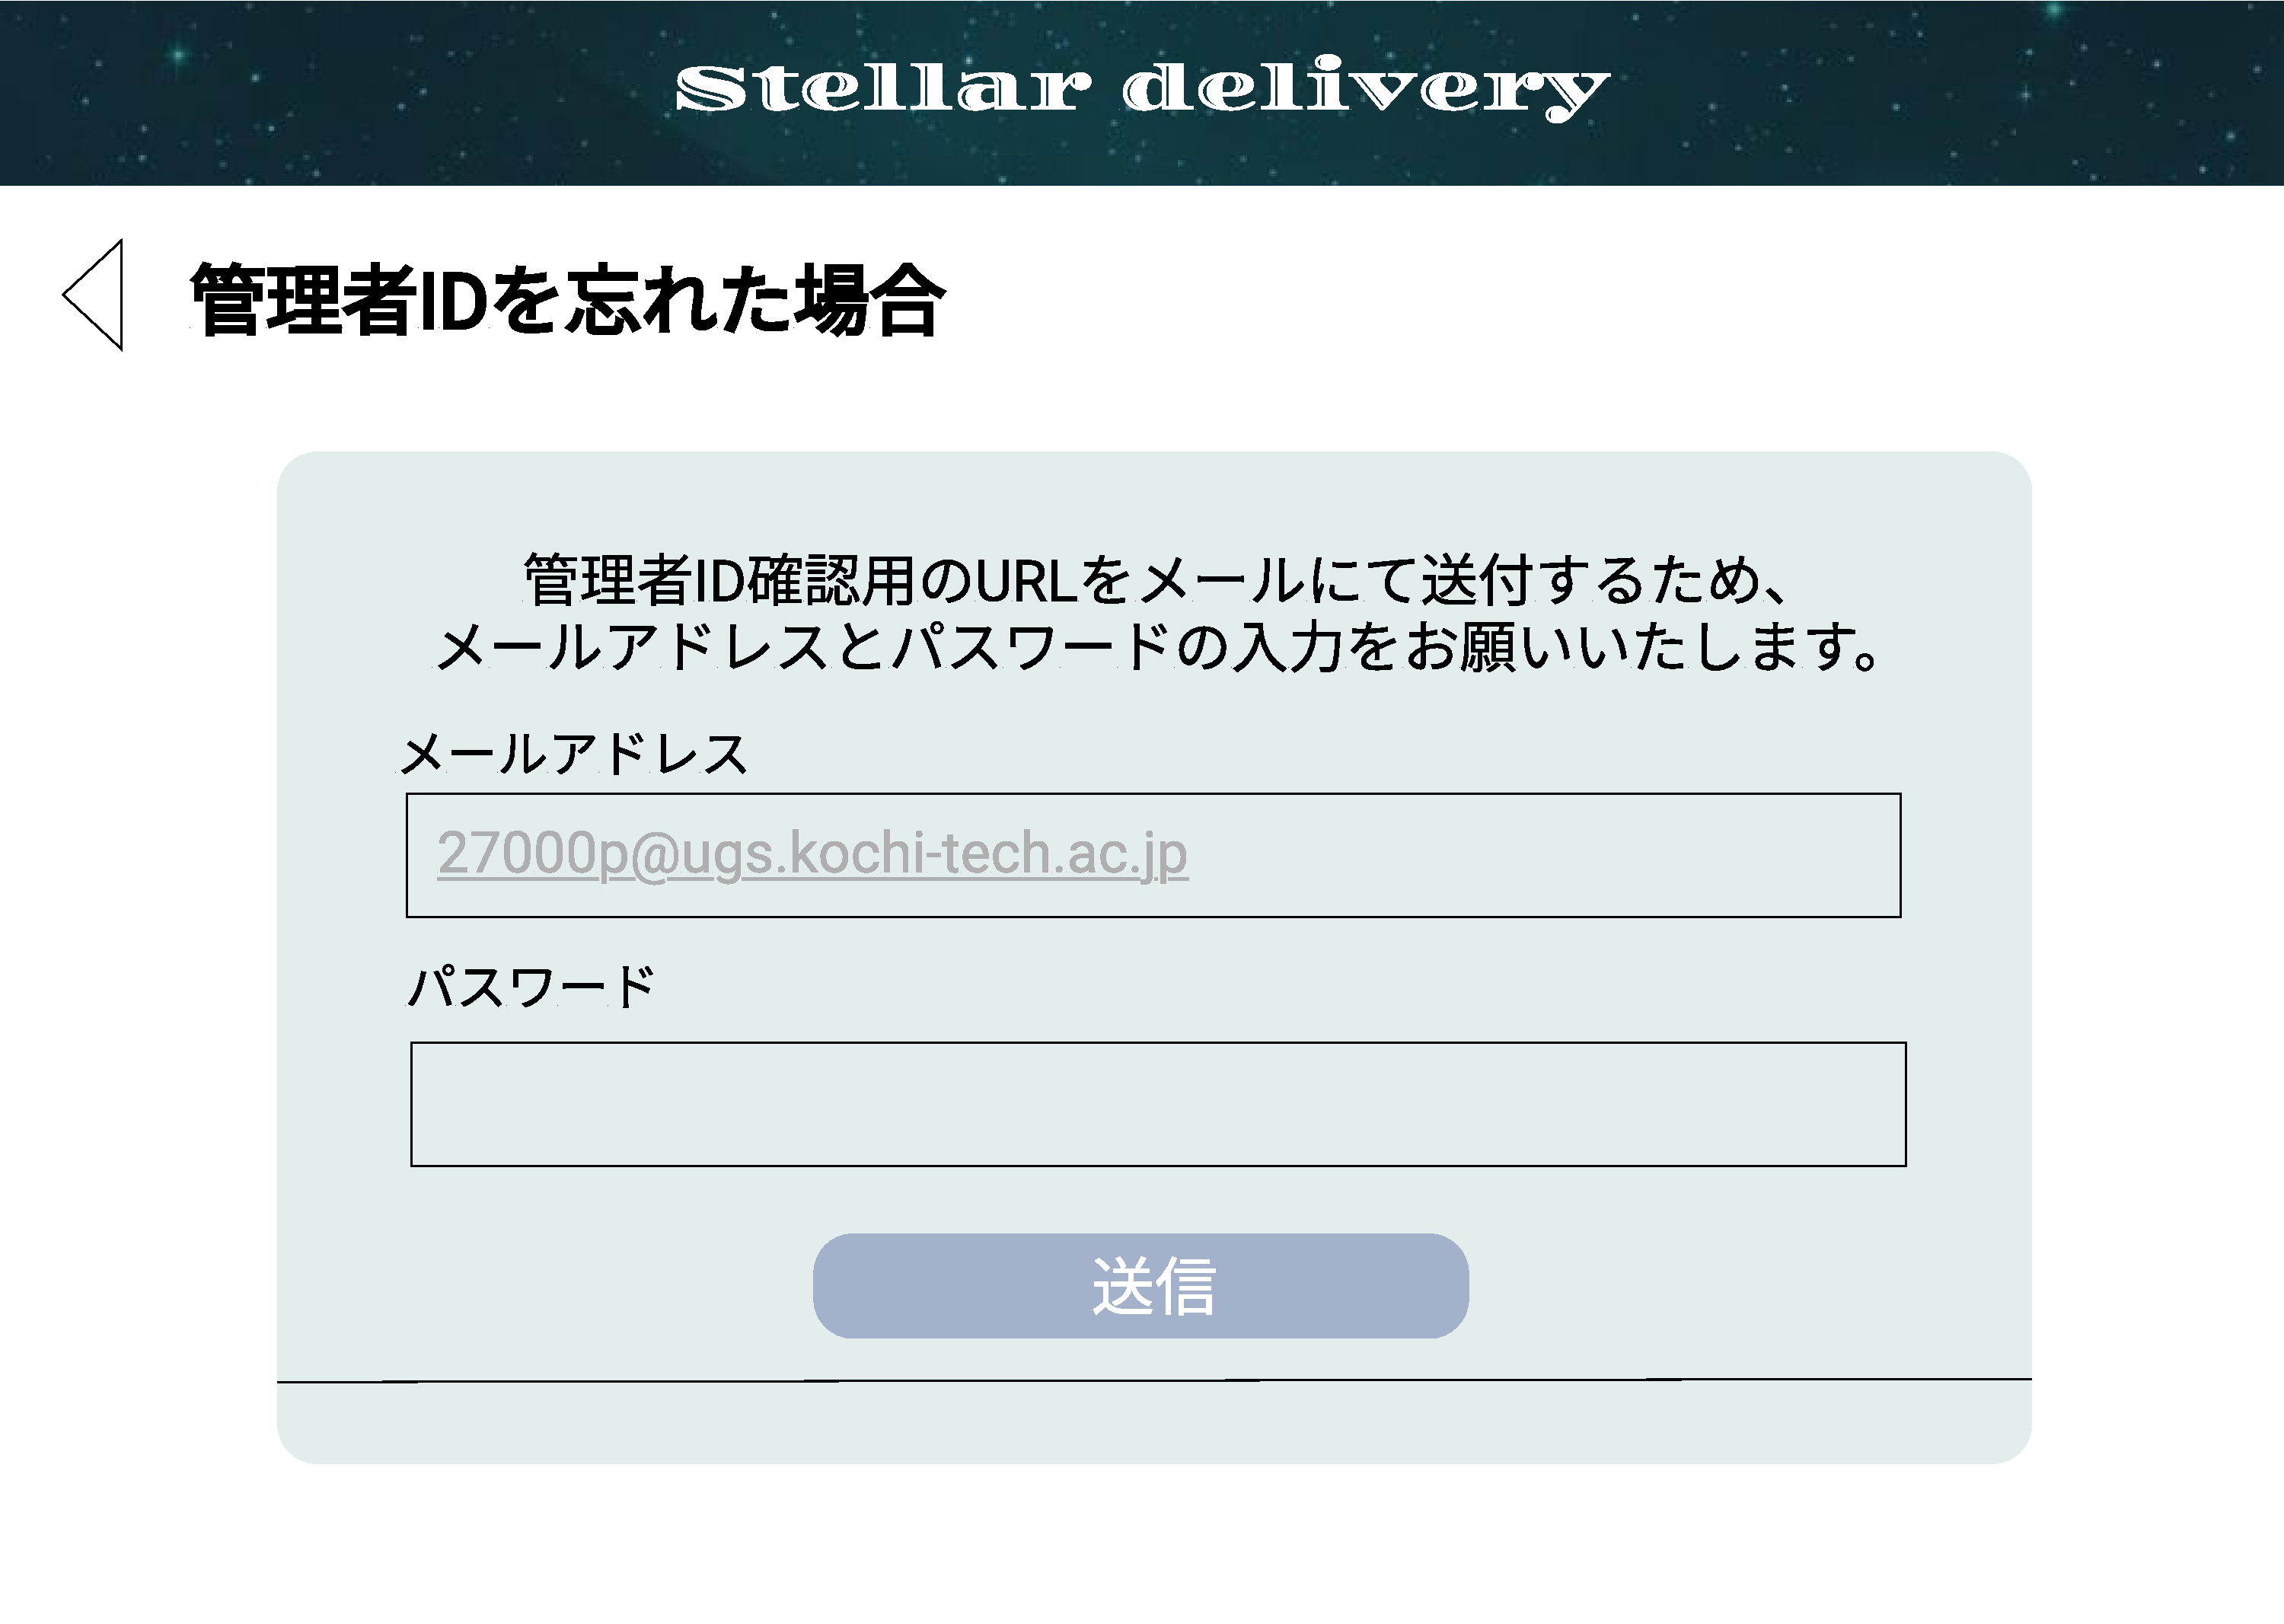
\includegraphics[width=0.75\textwidth]{./pic/administrator画面デザイン/0_ログイン/011_管理者ID場合のメールアドレス送信画面.pdf}
  \caption{管理者IDを忘れた場合}
  \label{fig:管理者IDを忘れた場合}
\end{figure}
\begin{figure}[H]
  \centering
  \includegraphics[width=0.75\textwidth]{./pic/administrator画面デザイン/0_ログイン/0111_管理者ID確認画面.pdf}
  \caption{管理者ID確認画面}
  \label{fig:管理者ID確認画面}
\end{figure}
\begin{figure}[H]
  \centering
  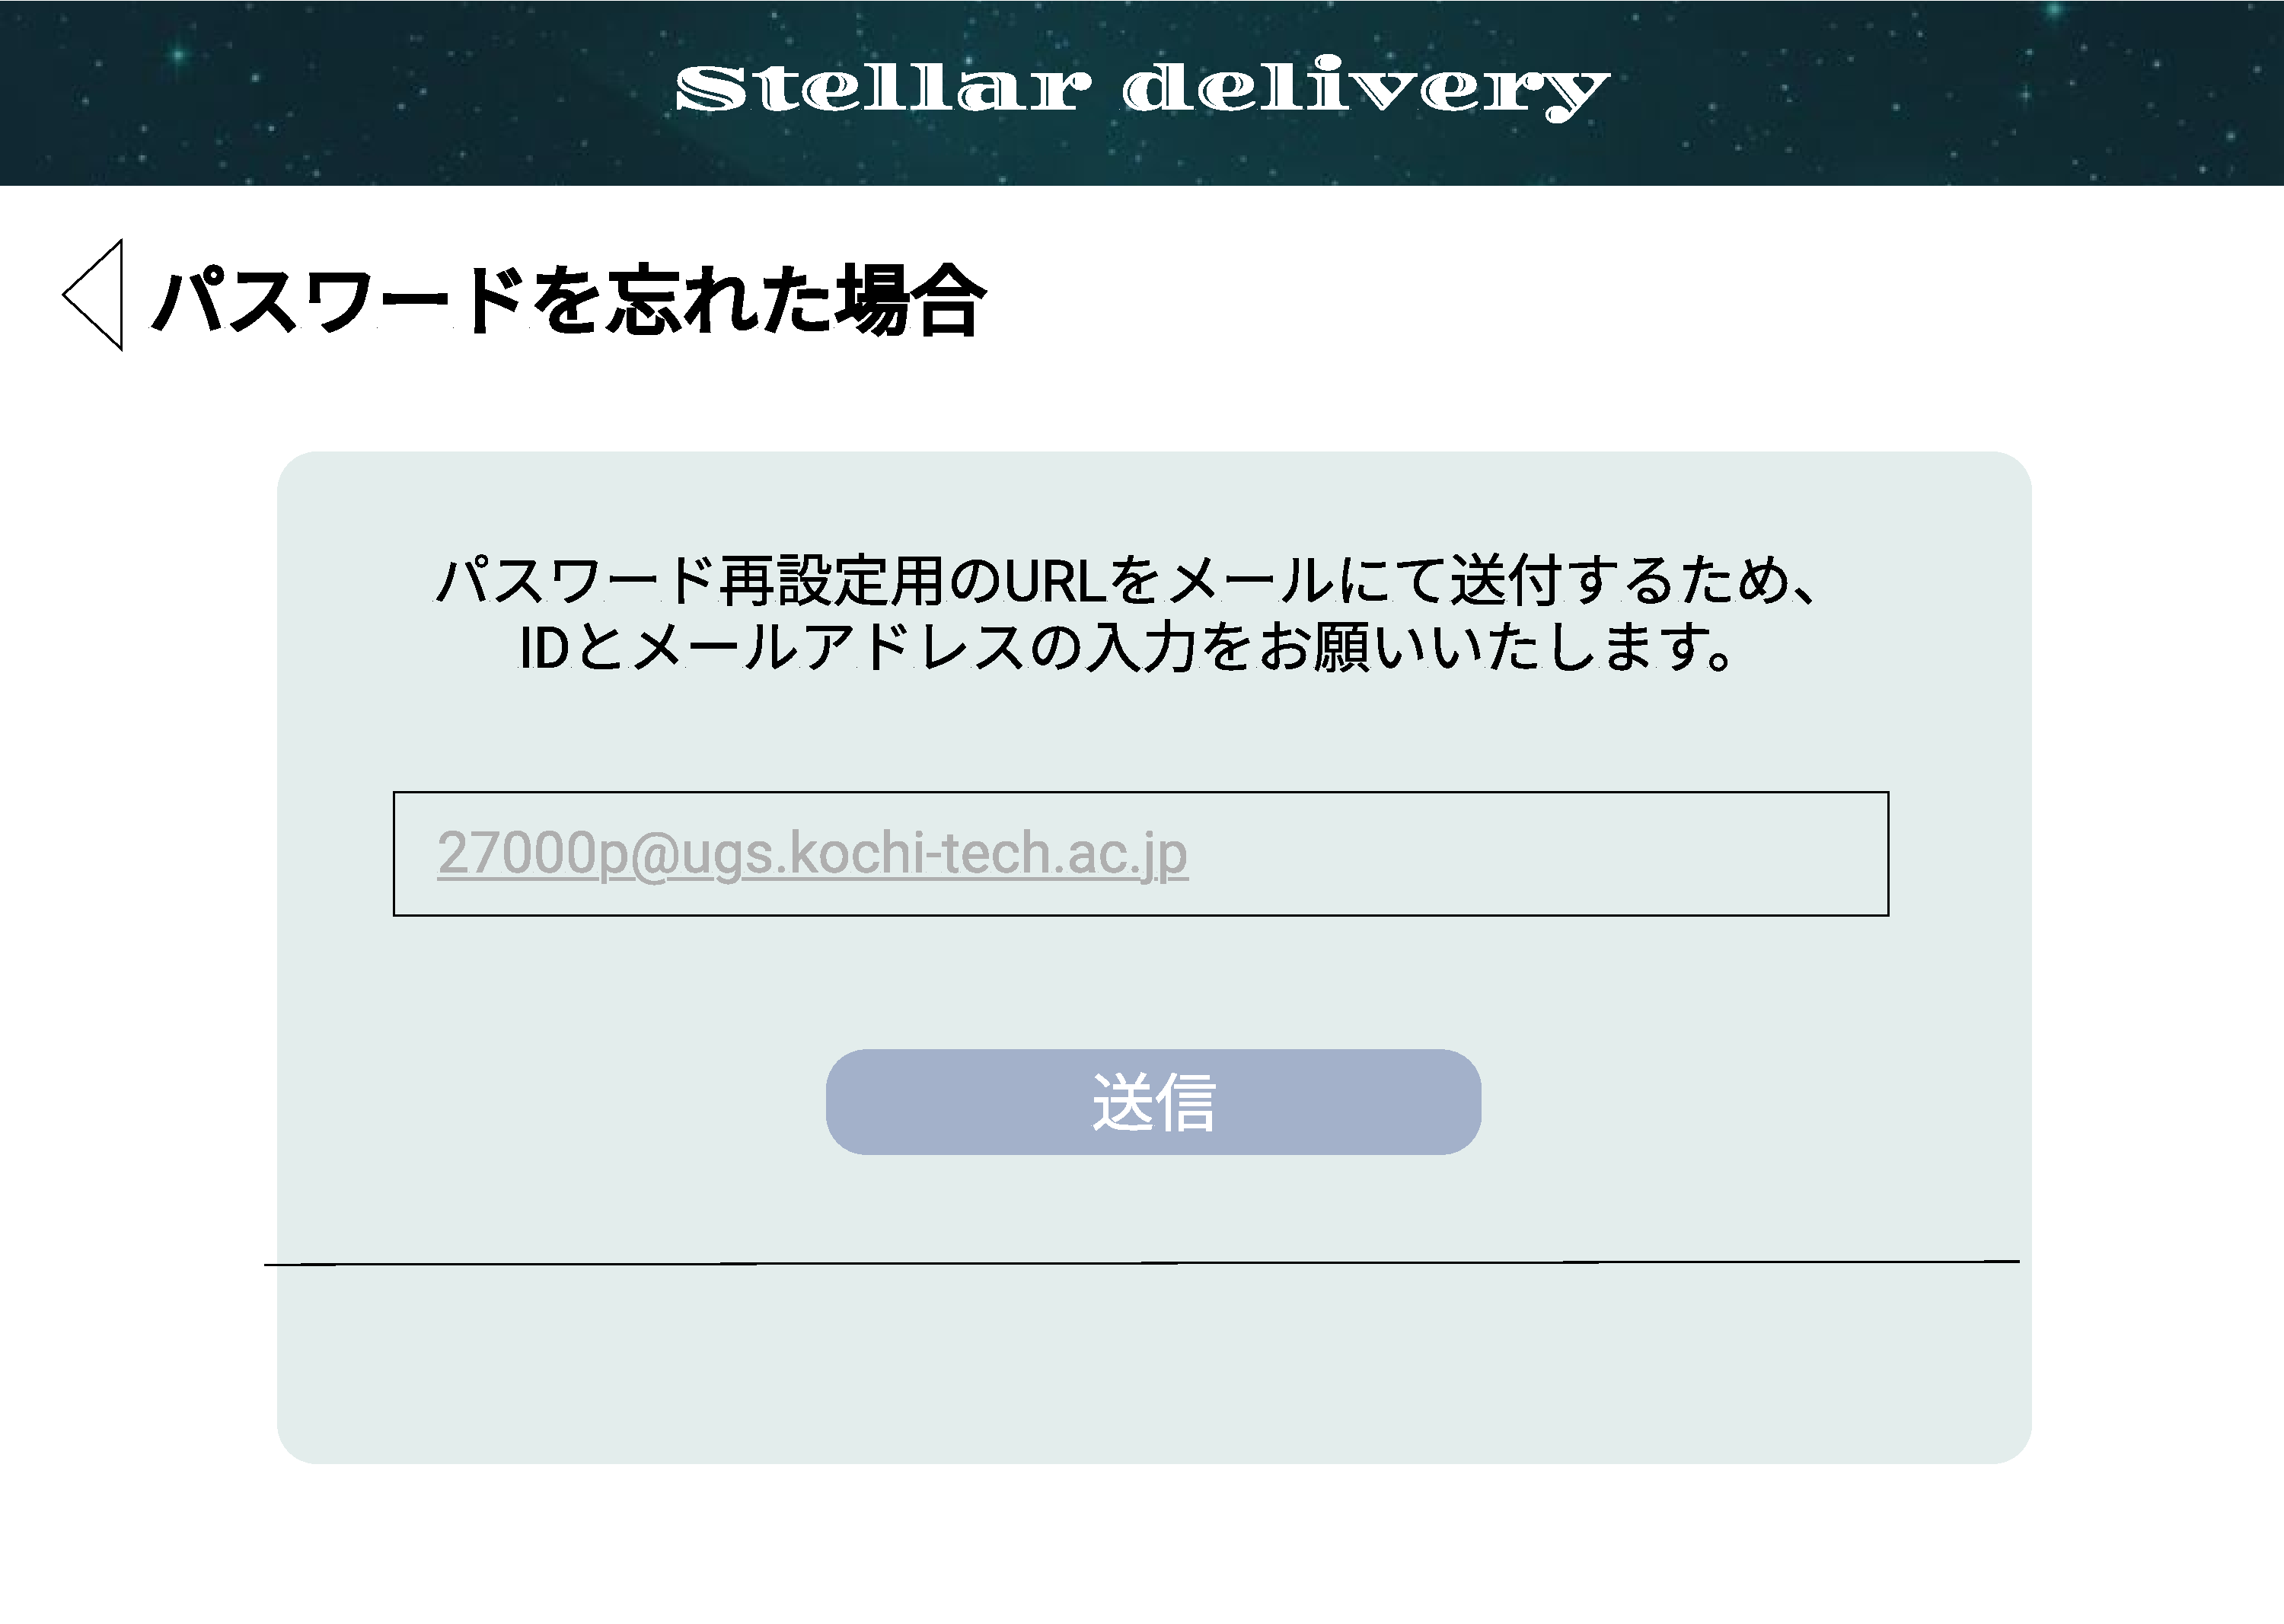
\includegraphics[width=0.75\textwidth]{./pic/administrator画面デザイン/0_ログイン/012_パスワードを忘れた場合のメールアドレス送信画面.pdf}
  \caption{パスワードを忘れた場合}
  \label{fig:パスワードを忘れた場合}
\end{figure}
\begin{figure}[H]
  \centering
  \includegraphics[width=0.75\textwidth]{./pic/administrator画面デザイン/0_ログイン/0121_パスワード再設定画面.pdf}
  \caption{パスワード再設定画面}
  \label{fig:パスワード再設定画面}
\end{figure}
